\chapter{Vita}

% Change the descriptions accordingly

{
\vfill

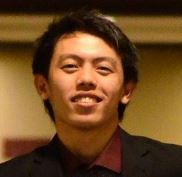
\includegraphics[width=0.2\columnwidth]{Chan}
 Zion Eric O. Chan is currently taking up his B.Sc. \degree \ studies and is in his 3rd academic year. He has made various projects consisting of software and hardware and the combination of both such as a line following robot and a sensor robot during his stay in the university. He is interested in the software side of the Computer Engineering program rather than the hardware side.
\vspace{5mm}

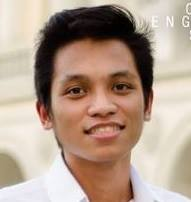
\includegraphics[width=0.2\columnwidth]{Comendador}
 Glenn Rommel P. Comendador is currently taking up his B.Sc. \degree \ studies and is in his 3rd academic year. He has also completed several projects such as the Batbot, the FM Radio, and the Line Following Robot. He is currently studying Data Communications, Digital Systems Design, Computer Systems Architecture and Microprocessor Systems in De La Salle University.
\vspace{5mm}

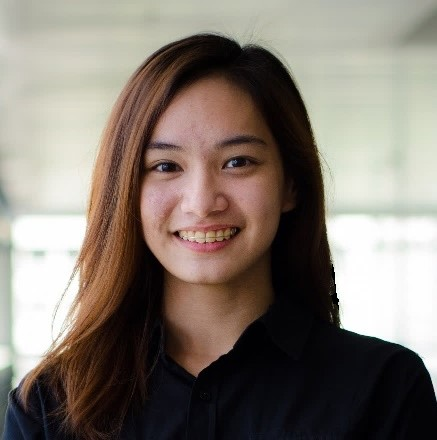
\includegraphics[width=0.2\columnwidth]{Garcia}
 Laureen Audrey R. Garcia is currently taking up her B.Sc. \degree \ studies and is in her 3rd academic year. She has completed various software and hardware related courses such as Switching Devices, Signal Processing, Advanced Electronics, and Principles of Communication. Her interest in engineering is more inclined to the study of Embedded and Real-Time Systems and Computer Hardware Architecture. 
\vspace{5mm}

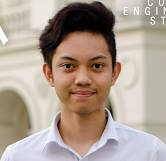
\includegraphics[width=0.2\columnwidth]{Fallar}
 Mac Excel S. Fallar is currently taking up his B.Sc. \degree \ studies and is in his 3rd academic year. He has completed multiple projects, mostly hardware and software offered in his course, during his stay in the University. He is proficient in Programming with the languages, C#, C++, and Java. Created a cloud database application for android mobile phones called Tap President, and helped create A line following robot, and a sensor robot. 
\vspace{5mm}

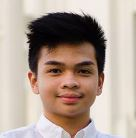
\includegraphics[width=0.2\columnwidth]{Lerit}
 Jose Mari Luis L. Lerit is currently taking up his B.Sc. \degree \ studies at the De la Salle University Manila and is now a 3rd year student. He has developed different skills and acquired knowledge in the field of computer engineering. He already completed some of his software and hardware courses which enabled him to create an android application, a line following mobot and a distance sensor mobot. His research interests focuses more on the hardware side, embedded system, microcontroller, microprocessor and computer system architecture.

\vfill
}